\documentclass[10pt, a5paper]{article}
\usepackage{pdfpages}
\usepackage{parallel}
\usepackage[T2A]{fontenc}
\usepackage{ucs}
\usepackage[utf8x]{inputenc}
\usepackage[polish,english,russian]{babel}
\usepackage{hyperref}
\usepackage{rotating}
\usepackage[inner=2cm,top=1.8cm,outer=2cm,bottom=2.3cm,nohead]{geometry}
\usepackage{listings}
\usepackage{graphicx}
\usepackage{wrapfig}
\usepackage{longtable}
\usepackage{indentfirst}
\usepackage{array}
\newcolumntype{P}[1]{>{\raggedright\arraybackslash}p{#1}}
\frenchspacing
\usepackage{fixltx2e} %text sub- and superscripts
\usepackage{icomma} % коскі ў матэматычным рэжыме
\PreloadUnicodePage{4}

\newcommand{\longpage}{\enlargethispage{\baselineskip}}
\newcommand{\shortpage}{\enlargethispage{-\baselineskip}}

\def\switchlang#1{\expandafter\csname switchlang#1\endcsname}
\def\switchlangbe{
\let\saverefname=\refname%
\def\refname{Літаратура}%
\def\figurename{Іл.}%
}
\def\switchlangen{
\let\saverefname=\refname%
\def\refname{References}%
\def\figurename{Fig.}%
}
\def\switchlangru{
\let\saverefname=\refname%
\let\savefigurename=\figurename%
\def\refname{Литература}%
\def\figurename{Рис.}%
}

\hyphenation{admi-ni-stra-tive}
\hyphenation{ex-pe-ri-ence}
\hyphenation{fle-xi-bi-li-ty}
\hyphenation{Py-thon}
\hyphenation{ma-the-ma-ti-cal}
\hyphenation{re-ported}
\hyphenation{imp-le-menta-tions}
\hyphenation{pro-vides}
\hyphenation{en-gi-neering}
\hyphenation{com-pa-ti-bi-li-ty}
\hyphenation{im-pos-sible}
\hyphenation{desk-top}
\hyphenation{elec-tro-nic}
\hyphenation{com-pa-ny}
\hyphenation{de-ve-lop-ment}
\hyphenation{de-ve-loping}
\hyphenation{de-ve-lop}
\hyphenation{da-ta-ba-se}
\hyphenation{plat-forms}
\hyphenation{or-ga-ni-za-tion}
\hyphenation{pro-gramming}
\hyphenation{in-stru-ments}
\hyphenation{Li-nux}
\hyphenation{sour-ce}
\hyphenation{en-vi-ron-ment}
\hyphenation{Te-le-pathy}
\hyphenation{Li-nux-ov-ka}
\hyphenation{Open-BSD}
\hyphenation{Free-BSD}
\hyphenation{men-ti-on-ed}
\hyphenation{app-li-ca-tion}

\def\progref!#1!{\texttt{#1}}
\renewcommand{\arraystretch}{2} %Іначай формулы ў матрыцы зліпаюцца з лініямі
\usepackage{array}

\def\interview #1 (#2), #3, #4, #5\par{

\section[#1, #3, #4]{#1 -- #3, #4}
\def\qname{LVEE}
\def\aname{#1}
\def\q ##1\par{{\noindent \bf \qname: ##1 }\par}
\def\a{{\noindent \bf \aname: } \def\qname{L}\def\aname{#2}}
}

\def\interview* #1 (#2), #3, #4, #5\par{

\section*{#1\\{\small\rm #3, #4. #5}}

\def\qname{LVEE}
\def\aname{#1}
\def\q ##1\par{{\noindent \bf \qname: ##1 }\par}
\def\a{{\noindent \bf \aname: } \def\qname{L}\def\aname{#2}}
}


\begin{document}

\title{Telepathy-skykit}%\footnote{Текст данных и последующих тезисов, кроме специально оговоренных случаев, доступен под лицензией Creative Commons Attribution-ShareAlike 3.0}

\author{Максим Мельников\footnote{Минск, Беларусь; \url{maxposedon@gmail.com}}}
\maketitle

\begin{abstract}
Telepathy-skykit, a Telepathy connection manager developed by the author, is presented. It implements Skype protocol support, and is based on Skype SDK for embedded development, known as SkypeKit. The project's goal is to use Skype without a `regular' desktop client, while using all features Telepathy provides: unified UI for all protocols, proper logging subsystem and Telepathy integration with Desktop Environment.
\end{abstract}

\subsection*{Telepathy}

Telepathy — программный каркас, используемый для создания программного обеспечения мгновенного обмена сообщениями, IP-телефонии или видеоконференций. Telepathy позволяет создавать приложения c помощью компонентов через систему межпроцессного взаимодействия D-Bus. При этом, logger, connection manager и UI работают в отдельных процессах.

\begin{figure}[t]
  \centering
  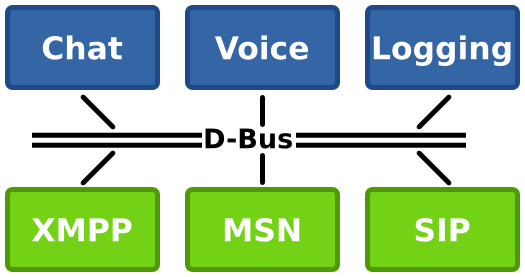
\includegraphics[width=6cm]{101_2013_w_Melnikau_tao}
\end{figure}

Для telepathy уже разработана поддержка основных протоколов:
\begin{itemize}
\item Gabble "--- Jabber/XMPP, включая Jingle;
\item Rakia "--- SIP;
\item Haze "--- обёртка над libpurple, внутренней библиотекой Pidgin; поддерживает все протоколы, с которыми умеет работать сам Pidgin.
\end{itemize}

С точки зрения UI, основными приложениями являются следующие два:
\begin{itemize}
\item Empathy, обладающий хорошей интеграция с Gnome и \linebreak Evalution Data Server;
\item KDE-Telepathy, предоставляющий аналогичную интеграцию с KDE.
\end{itemize}

Оба приложения поддерживают передачу звука и видео; также есть и другие, менее функциональные.

Также, уже разработаны следующие компоненты:
\begin{itemize}
\item logger "--- сервис отвечающий за хранение и предоставление логов по запросу
\item mission-control "--- управление аккаунтами
\end{itemize}

Таким образом, Telepathy "--- хорошо проработанный, модульный framework, содержащий много готовых унифицированных компонентов, и позволяющий которые легко добавлять новые или расширять существующие.

\subsection*{SkypeKit}
SkypeKit "--- коллекция утилит и API, которые позволяют разработать собственное устройство/приложение с поддержкой skype протокола: чат, аудио и видео. Причём разработан он с возможностью использования на большом количестве различных чипов, операционных систем и устройств, и является «безинтерфейсным».
\begin{figure}[b]
  \centering
  
\includegraphics[width=8cm]{101_2013_w_Melnikau_skypekit}
\end{figure}
Под Linux поддерживаются следующие аппаратные архитектуры: armv5le,
armv6le, armv7le, x86. Разработка может вестись на C++, C\#, java, python. При этом сам SkypeKit-демон не содержит UI, и для интеграции с системой может использовать ALSA, X11 OpenGL, либо GStreamer.

\subsection*{Skype в Telepathy}

Поддержка Skype в Telepathy до этого существовала в единственном виде: skype4pidgin "--- plugin для Pidgin (libpurle), поддерживающий Skype, который подключается как один из libpurple"=протоколов, через telepathy"=haze. Однако у неё существуют большие ограничения: отсутствие поддержки аудио и видео, а также части функциональности чата, vCard и других не базовых возможностей.

Альтернативный вариант, разработанный автором: telepathy"=sky\-kit "--- connection manager, реализующий поддержку Skype для Telepathy. При этом используется embedded-демон SkypeKit, который реализует поддержку протокола Skype, а telepathy"=skypekit при этом представляет собой лишь wrapper.

Для простоты реализации (прототипирования) был выбран Python. А для интеграции с Telepathy используется библиотека telepathy"=python, в которую была добавлена поддержка необходимого функциональности.

В данный момент реализованы:
\begin{itemize}
\item чат "--- самая базовая функциональность, общение один на один;
\item контакт-лист;
\item поддержка аватарок и карточка профиля (vCard).
\end{itemize}

Планы на будущее:
\begin{itemize}
\item конференции "--- очень часто используемая функциональность;
\item интеграция с OS "--- автоматический запуск демона при DBus-запросе и т.~д.;
\item аудио/видео звонки "--- хотя бы на уровне «proof of concept».
\end{itemize}
\begin{figure}[h]
  \centering
  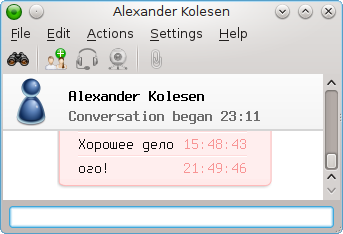
\includegraphics[width=6cm]{101_2013_w_Melnikau_ktpskype}
\end{figure}

\let\saverefname=\refname%
\def\refname{Полезные ссылки}%
\begin{thebibliography}{9}
\bibitem{meln1} \url{http://telepathy.freedesktop.org/wiki/}
\bibitem{meln2} \url{https://developer.skype.com/public/skypekit/}
\bibitem{meln3} \url{https://github.com/max-posedon/telepathy-skykit}
\bibitem{meln4} \url{https://github.com/max-posedon/telepathy-python}
\end{thebibliography}
\let\refname=\saverefname%

\end{document}




